\documentclass[10pt]{book}

\usepackage[T1]{fontenc}
\usepackage[utf8]{inputenc}
\usepackage[english]{babel}
\usepackage{geometry}
\usepackage{graphicx}
\usepackage[pdfa=true]{hyperref}
\usepackage{cite}
\usepackage{listings}
\usepackage[printonlyused,withpage]{acronym}
\usepackage{siunitx}
\usepackage{multirow}
\usepackage{setspace}
\usepackage{xcolor}
\usepackage{listings}
\usepackage{tabularx}
\usepackage{marvosym}

% OWN packages
\usepackage{wrapfig}
\usepackage{cleveref}

%--- pdf/a format ----
% insert metadata about the document here
\RequirePackage{filecontents}
\begin{filecontents*}{\jobname.xmpdata}
\Title{Bachelor thesis}
\Author{Robin William hundt}
\Language{en-US}
\Subject{The abstract, or short description.}
\Keywords{keyword1\sep keyword2\sep keyword3}
\end{filecontents*}
\usepackage{colorprofiles}
\usepackage[a-1b,mathxmp]{pdfx}[2018/12/22]
\usepackage[T1]{fontenc}
\hypersetup{pdfstartview=}


%
% This is the official thesis template of
% the Institute of Computer Science at the
% Georg-August-University of Göttingen
%
%      author: kellner@cs.uni-goettingen.de
% last update: 17/02/2015
%
% If you find any sort of mistake please let me know
% so that it can be fixed in future releases.
%


%--- include custom commands ---
%
% own commands
%

%double empty page
\newcommand \myemptypage {
    \clearpage
    \thispagestyle{empty}
    \null
    \cleardoublepage
}

%create abstract environment that is not available in latex book style
\newcommand\abstractname{Abstract}
\newenvironment{abstract}{%
    \begin{center}%
        \normalfont\Large\bfseries \abstractname
    \end{center}%
    \it%
    }
    {}


%--- include general configuration ---
%
% general configuration
%

% Palatino font as serif font
\usepackage{palatino}
\linespread{1.05}
% Helvatica font as sans-serif
\usepackage{helvet}
% Use microtype to improve typesetting
\usepackage{microtype}

%set page margin for DIN A4
\geometry{a4paper, left=2.5cm, right=2.5cm, top=4cm, 
          bottom=5cm, bindingoffset=1cm}

%makes TeX less fussy about line breaking
\sloppy

% Replacement for changing parskip and parindent directly
\usepackage{parskip}

%1.5 spacing
\onehalfspacing
{}

%% Make chapter heading smaller
%\usepackage{titlesec}
%\titleformat{\chapter}[display]
%  {\LARGE\bf}{\chaptertitlename\ \thechapter}{10pt}{\huge\bf}

% This are much nicer chapter headings than the original one and even smaller
\usepackage{titlesec, blindtext, color}
\definecolor{gray75}{gray}{0.75}
\newcommand{\hsp}{\hspace{20pt}}
\titleformat{\chapter}[hang]{\LARGE\bfseries}{\thechapter\hsp\textcolor{gray75}{|}\hsp}{0pt}{\LARGE\bfseries}


%define some colors
\definecolor{darkblue}{rgb}{0.0,0.0,0.5}
\definecolor{grey}{rgb}{0.8,0.8,0.8}
\definecolor{lightgrey}{rgb}{0.95,0.95,0.95}

%set listing style properties for python
\lstset{language=Python,
    basicstyle=\footnotesize\ttfamily,
    captionpos=b,
    frame=tb,
    commentstyle=\color{gray} \bfseries,
    stringstyle=\color{green}\ttfamily,
    keywordstyle=\color{darkblue}\bfseries,
    breaklines=true,
    aboveskip=10mm,
    belowskip=10mm,
    showstringspaces=false
    numbers=left,
    %stepnumber=5,
    numberstyle=\tiny,
    numbersep=5pt
}


%override reference title and listings title
\renewcommand \bibname{References}
\renewcommand{\lstlistlistingname}{List of Listings}




%--- basic document configuration ---
\newcommand{\mytype}{Bachelor's Thesis}
%\newcommand{\mytype}{Master's Thesis}

\newcommand{\mycourse}{Applied Computer Science}
%\newcommand{\mycourse}{Internet Technologies and Information Systems}

\newcommand{\mytitle}{My Title}
\newcommand{\myauthor}{Robin William Hundt}
\newcommand{\mydepartment}{Institute of Computer Science}
\newcommand{\mysubmissiondate}{09. May 2020}
\newcommand{\mythesisid}{201x-xx} %assigned by examination office
\newcommand{\myfirstsupervisor}{Prof. Dr. Burkhard Morgenstern}
\newcommand{\mysecondsupervisor}{Dr. Peter Meinicke}


\begin{document}

 \pagenumbering{roman}
    \setcounter{page}{1}

   %--- cover page ---
   %
% title page
%

\begin{titlepage}
    %--- logo ---
    \normalsize
    \begin{tabularx}{\textwidth}{lXr}
        \multirow{2}{*}{
\includegraphics[width=6.5cm]{images/goe-logo.jpg}} 
        & & ISSN 1612-6793\\
    \end{tabularx}

    %default settings for the rest
    \large
    \centering

    \vspace{3cm}

    \textbf{\LARGE \mytype}\\

    submitted in partial fulfillment of the\\
    requirements for the course ``\mycourse''

    \vspace{2cm}

    \textbf{\LARGE \mytitle}

    \vspace{2cm}

    \myauthor

    \vspace{2cm}

    \mydepartment

    \vspace{2cm}

    Bachelor's and Master's Theses\\
    of the Center for Computational Sciences\\
    at the Georg-August-Universität Göttingen

    \vspace{0.2cm}

    \mysubmissiondate


    %--- new page ---
    \myemptypage
    \clearpage
    \thispagestyle{empty}
    \null
    \flushleft
    \onehalfspacing
    \normalsize

    \vspace{12cm}

    Georg-August-Universität Göttingen\\
    Institute of Computer Science\\[3ex]
    Goldschmidtstraße 7\\
    37077 Göttingen\\
    Germany\\[3ex]

    \begin{tabular}{@{}ll}
        \Telefon & +49 (551) 39-172000\\
        \fax & +49 (551) 39-14403\\
        \Letter & \href{mailto:office@informatik.uni-goettingen.de}{office@informatik.uni-goettingen.de}\\
        \Mundus & \url{www.informatik.uni-goettingen.de}\\
    \end{tabular}

    \vspace{1.0cm}

    \begin{tabular}{@{}ll}
        First Supervisor: & \myfirstsupervisor\\
        Second Supervisor:& \mysecondsupervisor\\
    \end{tabular}

    \clearpage
\end{titlepage}


   \myemptypage

    %--- statement page ---
    \thispagestyle{empty}

\null
\vspace{16.5cm}

\rule{\textwidth}{0.4pt}

I hereby declare that I have written this thesis independently without any help from others and without the use of documents or aids other than those stated. I have mentioned all used sources and cited them correctly according to established academic citation rules.

\vspace{0.2cm}

Göttingen, \mysubmissiondate

    \myemptypage

    %--- abstract ---
    \clearpage\phantomsection\pdfbookmark{\abstractname}{abstract}
    \thispagestyle{empty}
    \begin{abstract}
    \textbf{Motivation}\\
    \begin{itemize}
    	\item sequencing data is ever increasing
    	\item MSA, while being an indispensable part of biology and bioinformatics research is a computationally very expensive problem
    	\item in need of new heuristics and algorithms which can be used to calculate MSA with constrained resources
    	\item earlier work examined the feasibility of an alignment approach based on spaced word matches and consistency checks in conjuction with GABIOS-LIB
    	\item this work provides an implementation and evaluation of this approach
    \end{itemize}
    
    \textbf{Results}\\
    
    
\end{abstract}


    \myemptypage

    %reset acronyms after abstract
    \acresetall

    %--- table of contents ---
    \clearpage\phantomsection\pdfbookmark{\contentsname}{toc}
    \tableofcontents
    \myemptypage

    %--- list of figures ---
    %\listoffigures
    %\myemptypage

    %--- list of tables ---
    %\listoftables
    %\myemptypage

    %--- list of listings ---
    %\lstlistoflistings
    %\myemptypage

    %--- list of acronyms ---
    %\chapter*{List of Abbreviations}

\begin{acronym}[myacronyms]
    \acro{FYI}{For Your Information}    
\end{acronym}

    %\myemptypage


    %arabic page numbers
    \pagenumbering{arabic}
    \setcounter{page}{1}
    
    %--- chaper 1..n ---
    \chapter{Introduction}
    \myemptypage

    \chapter{Basics}

\begin{itemize}
	\item what is a MSA and for what is it important?
	\item math def of consistency and msa
\end{itemize}

\section{Multiple sequence alignment}



As a generalisation of pairwise sequence alignments, multiple sequence alignments are the basis for numerous further analyses such as "inferring phylogenetic relationships, homology search of functional elements, classification of proteins, designing detection markers" \cite[pg. 3]{Russell2016}. In contrast to the pairwise alignment problem, aligning an arbitrary number of sequences is a NP-complete problem, when formulated as the maximisation (or minimisation) of an objective function \cite[pg. 172]{Russell2016}.\\
The classical formulation of the problem is based upon a model of evolution where single residues get inserted, deleted or substituted. Since an insertion in one sequence is indistinguishable of a deletion in another one, these two operations are commonly viewed as one and referred to as an \textit{indel}. The goal is then to insert gaps, representing an indel and denoted as \textit{'-'} into the sequences, such that they have the same length and a given score function is maximal for the produced Alignment. These aligned sequences are usually displayed as a table of residues and gap characters as seen in \cref{tab:msa-example}\cite{Russell2016}. 

\begin{table}[h]
\centering
\begin{tabular}{l c c c c c c c c c c c c c c c c c c c c c c c c c c c c c c c c c c c c}
	seq1 & L&L&I&R&N&L&I&Q&V&-&V&K&S&V&-&-&-&- \\
	seq2 & L&L&I&R&K&L&I&D&V&-&V&R&T&V&-&-&-&- \\
	seq3 & L&L&I&R&Q&L&I&D&V&-&I&K&T&V&-&-&-&- \\
	seq4 & L&L&I&-&-&-&-&Q&M&A&D&Q&Y&L&P&E&T&L \\
\end{tabular}
\caption{Example of multiple sequence alignment. The gap symbol '-' represents an insertion or deletion (often combined as \textit{indel}).}
\label{tab:msa-example}
\end{table}


\section{Mathematical notion of Consistency and Alignments}
A more formal definition of the term \textit{Alignment} is based upon the work by Morgenstern et al. \cite{morgenstern1996multiple} and Abdedda{\"\i}m \cite{abdeddaim2000speeding}. The following definitions constitute a condensed formalization of the one provided in the preliminary work to this thesis \cite{hundt2020praktkium}.\\ 
% TODO so formulieren dass klar ist, dass das größtenteils verbatim ist

Let $S_i$ be a Sequence over an Alphabet, e.g. DNA, Amino Acids, etc., and $S := \{S_1, ..., S_n\}$ a set of Sequences.\\

\begin{mydef}[Site]
	A site $x = [i,p]$ represents the $p$-th position in the $i$-th sequence and $X$ is the set of all sites for $S$.\\
	The function 
	\begin{align*}
	seq: &X \rightarrow \mathbb{N}\\
	&x \mapsto i
	\end{align*}
	maps a site to its corresponding sequence. Whereas the function
	\begin{align*}
	pos: &X \rightarrow \mathbb{N}\\
	&x \mapsto p
	\end{align*}
\end{mydef}
maps a site to its position.
\begin{mydef}[Ordering of Sites]
	For $x = [i, p], x'=[i', p'] \in X$ we define $x \preceq y$ if and only if $i = i'$ and $p \leq p'$.\\
	The relation $\preceq$ is a partial ordering on $X$.
\end{mydef}


\begin{mylemma}[Extension of binary relation to quasi order relation]
	Let $A$ be a reflexive binary relation on some set $X$ and $R$ any binary relation on $X$.\\
	The transitive closure $\preceq_R :=(A\cup R)^t$ is a quasi order relation on $X$.\\
	\label{lem:extension-quasiorder}
\end{mylemma}

As per lemma \ref{lem:extension-quasiorder} we extend $\preceq$ to the quasi partial order $\preceq_R$ by taking the transitive closure of the union of $\preceq$ and $R$. Consequently $u\preceq v$, $vRw$, $w\preceq x$, $xRy$ and $y\preceq z$ from which follows that $y \preceq_R z$.

\begin{mydef}[Consistency]
	Let $R$ be a binary relation on a set of sites $X$. $R$ is consistent if for $x, y \in X$ where $seq(x) = seq(y)$
	\begin{equation*}
	x \preceq_R y \implies x \preceq y
	\end{equation*}
	
	
	holds. Additionally a set $\{R_1, ..., R_n\}$ of binary relations on $X$ is consistent if $\cup_i R_i$ is consistent.
	
	\label{def:consistency}
\end{mydef}

\begin{mydef}[Alignment]
	An alignment (or partial alignment) $A$ is a consistent equivalence relation on the set of sites $X$ for a set of sequences $S$. 
	\label{def:alignment}
\end{mydef}


\begin{figure}[ht]
	\tikzset{SeqNode/.style={circle, draw, fill=black, inner sep=0pt, minimum width=4pt}}
	\centering
	\begin{tikzpicture}[thick]
	
	\draw 
	(0, 0) node [] {$S_1$}
	(1,0) -- (2,0)
	\foreach \x in {2, ..., 12}
	{
		(\x,0) node[SeqNode] {} -- (\x+1,0)
	}
	(0, 1) node [] {$S_2$}
	(1, 1) -- (2,1)
	\foreach \x in {2,..., 12}
	{
		(\x, 1) node[SeqNode] {} -- (\x+1,1)
	}
	(0, 2) node [] {$S_3$}
	(1, 2) -- (2,2)
	\foreach \x in {2,..., 12}
	{
		(\x, 2) node[SeqNode] {} -- (\x+1,2)
	};
	\foreach \x in {2, ..., 5}
	{
		\draw[-, line width=1.5] (\x,0) -- (\x + 1,1);
	}
	\foreach \x in {5, ..., 8}
	{
		\draw[-, line width=1.5] (\x,1) -- (\x - 1,2);
	}
	\foreach \x in {8, ..., 10}
	{
		\draw[-, line width=1.5] (\x,1) -- (\x + 2 ,0);
	}
	\end{tikzpicture}
	\caption{Example of a consistent equivalence relation $A$ on the set of sites $X$ for $S=\{S_1, S_2, S_3\}$. Connections between nodes $x,y$ represent represent a relation $xAy$.}
	\label{fig:consistent-alignment}
\end{figure}
    \myemptypage

    \chapter{Prior Work}

	\myemptypage

    \chapter{Algorithm}
\label{chap:algorithm}
This thesis provides an implementation and improvement of the alignment algorithm proposed in \cite{hundt2020praktkium}.

% TODO the algorithms input and output data needs
% to be cleaned up

\begin{algorithm}[H]
	\DontPrintSemicolon
	\KwData{Sequences $S = {S_1, ..., S_N}$}
	\KwData{Pattern set $P = {P_1, ..., P_M}$}
	\KwResult{Partial Alignment $A$ }
	\SetKwData{ma}{micro\_alignments}
	\SetKwData{pa}{partial\_alignment}
	\SetKwFunction{sort}{sort\_by\_score\_descending}
	\SetKwFunction{incons}{is\_inconsistent}
	\SetKwFunction{findspam}{find\_spaced\_word\_matches}
	\SetKwFunction{addsite}{add\_site\_pair}
	\SetKwFunction{notaligned}{not\_aligned}
	
	
	\pa $\leftarrow$ $\{\}$\;
	
	\ma $\leftarrow$ \findspam{$S$, $P$}\;
	\ma.\sort{}\;
	
	\ForEach{ma in \ma}{
		\If{\incons{ma, \pa}}{
			continue\;
		}
		\ForEach{site\_pair in ma}{
		\If{\pa.\notaligned{site\_pair}} {
				\pa.\addsite{site\_pair}\;	
			}
		}
	}	
	\Return \pa\;
	
	\caption{\bf{align($S$, $P$)}}
	\label{alg:align}
\end{algorithm}

Observation 3 of \cite{abdeddaim1997incremental, abdeddaim2000speeding} gave rise to following algorithm which can be improved

\begin{algorithm}[h]
	\DontPrintSemicolon
	\KwData{Consistent site pair $a,b \in X$ to align}
	\KwData{Partial Alignment $A$}
	\KwResult{Partial Alignment $A' = A \cup \{(a, b)\}$ }

	\SetKwFunction{min}{min}
	\SetKwFunction{max}{max}
	
	\tcp{Clone the old pred and succ values}
	$pred \leftarrow$ $pred_A$\;
	$succ \leftarrow$ $succ_A$\;
	
	\tcp{Update the successor frontier}
	\ForEach {$x \in X$} {
		\For {$i \leftarrow 1$ \KwTo $N$} {
			\If{$ x \preceq_{A} a$}{
				$succ_A[x, i]$ $\leftarrow$ \min{$succ[x, i], succ[b, i]$}
			}
			\ElseIf{$ x \preceq_{A_i} b$} {
				$succ_A[x, i]$ $\leftarrow$ \min{$succ[x, i], succ[a, i]$}
			}
			\Else{
				$succ_A[x, i] \leftarrow succ[x, i]$
			}
		}
	}
	
	\tcp{Update the predeccessor frontier}
	\ForEach {$x \in X$} {
		\For {$i \leftarrow 1$ \KwTo $N$} {
			\If{$ x \succeq_{A} a$}{
				$pred_A[x, i]$ $\leftarrow$ \max {$pred[x, i], pred[b, i]$}
			}
			\ElseIf{$ x \succeq_{A_i} b$} {
				$pred_A[x, i]$ $\leftarrow$ \max{$pred[x, i], pred[a, i]$}
			}
			\Else{
				$pred_A[x, i] \leftarrow pred[x, i]$
			}
		}
	}
	\caption{add\_site\_pair(x, y) as proposed in \cite{hundt2020praktkium}}
	\label{alg:add-site-pair}
\end{algorithm}


TODO Question: Why are \ref{alg:add-site-pair} and \ref{alg:add-site-pair-revised} equivalent?

\begin{algorithm}[h]
	\DontPrintSemicolon
	\KwData{Consistent site pair $a,b \in X$ to align}
	\KwData{Partial Alignment $A$}
	\KwResult{Partial Alignment $A' = A \cup \{(a, b)\}$ }
	
	\tcp{Update the successor frontier}
	\For {$i \leftarrow 1$ \KwTo $N$} {
		\For{$j \leftarrow 1$ \KwTo $N$}{
			\For{$p \leftarrow pred_A[a][i]$ \KwTo $1$}{
				$u \leftarrow Site [p, i]$\;
				\If{not $succ_A[b][j] < succ_A[u][j]$}{
					\bf{break}\;
				}
%			Why is u predecessor of a? needed for Observation 3
% 			u is pred of a because u is <= pred[a][i] 
				$succ_A[u][j] \leftarrow succ_A[b][j]$\;
			}
		}
		
	}

	\tcp{Update the predecessor frontier}
	\For {$i \leftarrow 1$ \KwTo $N$} {
		\For{$j \leftarrow 1$ \KwTo $N$}{
			\For{$p \leftarrow succ_A[b][i]$ \KwTo $len(S_i)$}{
				$u \leftarrow Site [p, i]$\;
				\If{not $pred_A[a][j] > pred_A[u][j]$}{
					\bf{break}\;
				}
				$pred_A[u][j] \leftarrow pred_A[a][j]$\;
			}
		}
		
	}

	\caption{add\_site\_pair(x, y) as proposed by Abdedda{\"\i}m \cite{abdeddaim1997incremental}}
	\label{alg:add-site-pair-revised}
\end{algorithm}


\begin{algorithm}[h]
	\DontPrintSemicolon
	\KwData{Consistent site pair $a,b \in X$ to align}
	\KwData{Index $nn$ of alignment set that was merged from alignment sets of $a$ and $b$}
	\KwData{Successor frontier $succ$}
	\KwData{Predecessor frontier $pred$}
	\KwData{$alig\_set$ matrix, mapping an alignment set and sequence to a position}
	\KwData{$pred\_alig\_set\_pos$ mapping a sequence and position to the index of the next predecessor alignment set of that site}
	\KwResult{Updated tranisitivity frontiers $succ$ and $pred$}
	\SetKwFunction{push}{push}
	
	\tcp{Update the successor frontier}
	$frontier\_ops \leftarrow [\ ]$
	
	\For {$i \leftarrow 1$ \KwTo $N$} {
		\If{$left_a[i] == left_b[i]$}{
			\bf{continue}\;
		}
		\For{$j \leftarrow 1$ \KwTo $N$}{
			$k \leftarrow pred_A[nn,\ i]$\;
			\If{$k > 0$ \bf{and} $k == alig\_set[nn,\ i]$}{
				$k \leftarrow pred\_alig\_set\_pos[i,\ k]$\;	
			}
			\While{$k > 0$}{
				$n \leftarrow alig\_set\_nbr[i,\ k]$\;
				\If{$succ[n,\ j] > succ[nn,\ j]$}{
					$frontier\_ops$.\push($[n,\ j,\ succ[nn,\ j]]$)\;
					$k \leftarrow pred\_alig\_set\_pos[i,\ k]$\;
				} 
				\Else{
					\bf{break}\;
				}
			}
		}
	}
	
	\ForEach{$[n,\ j,\ new\_front] \in frontier\_ops$}{
		$succ[n,\ j] \leftarrow new\_front$\;
	}
	\BlankLine
	\tcp{Update the predecessor frontier}
	\tcp{ommited for brevity}
	
	\caption{revised add\_site\_pair(x, y) based on GABIOS-LIB implementation in Dialign2.2 \cite{abdeddaim2000speeding}}
	\label{alg:add-site-pair-revised-2}
\end{algorithm}

As pointed out in \cite{abdeddaim2000speeding, hundt2020praktkium} partitioning the aligned sites into equivalence classes respective to the relation of whether two sites aligned allows for a more compact storage and efficient update of the transitivity frontiers due to them coinciding for every site in an eq class.\\
\\
\begin{figure}[ht]
	\tikzset{SeqNode/.style={circle, draw, fill=black, inner sep=0pt, minimum width=4pt}}
	\centering
	\begin{tikzpicture}[thick]
	
	\draw 
	(0, 0) node [] {$S_1$}
	(1,0) -- (2,0)
	\foreach \x in {2, ..., 6}
	{
		(\x,0) node[SeqNode] {} -- (\x+1,0)
	}
	(0, 1) node [] {$S_2$}
	(1, 1) -- (2,1)
	\foreach \x in {2,..., 6}
	{
		(\x, 1) node[SeqNode] {} -- (\x+1,1)
	}
	(0, 2) node [] {$S_3$}
	(1, 2) -- (2,2)
	\foreach \x in {2,..., 6}
	{
		(\x, 2) node[SeqNode] {} -- (\x+1,2)
	}
	(3, 0)+(-0.2, 0.2) node [] {a}
	(4, 1)+(-0.2, 0.2) node [] {b}
	(4, 2)+(-0.2, 0.2) node [] {c}
	(5, 2)+(0, 0.3) node [] {[3, 4]};
	\draw[-, line width=1.5] (3,0) -- (4,1);
	\draw[-, line width=1.5] (4,1) -- (4,2);
	\end{tikzpicture}
	\caption{TODO}
	\label{fig:eq-classes}
\end{figure}


While the algorithm \ref{alg:add-site-pair} for maintaining a transitive closure when adding a pair of sites $(a, b)$ into a partial alignment works, it is far from optimal. 


\begin{figure}[ht]
	\tikzset{SeqNode/.style={circle, draw, fill=black, inner sep=0pt, minimum width=4pt}}
	\centering
	\begin{tikzpicture}[thick]
	
	\draw 
	(0, 0) node [] {$S_1$}
	(1,0) -- (2,0)
	\foreach \x in {2, ..., 6}
	{
		(\x,0) node[SeqNode] {} -- (\x+1,0)
	}
	(0, 1) node [] {$S_2$}
	(1, 1) -- (2,1)
	\foreach \x in {2,..., 6}
	{
		(\x, 1) node[SeqNode] {} -- (\x+1,1)
	}
	(2, 0)+(-0.2, 0.2) node [] {a}
	(3, 1)+(-0.2, 0.2) node [] {b};
	\draw[-,dotted, line width=1.5] (2,0) -- (3,1);
	\draw[-, line width=1.5] (4,0) -- (4,1);
	\end{tikzpicture}
	\caption{TODO}
	\label{fig:unnecessary-cmp}
\end{figure}




\Cref{fig:unnecessary-cmp} displays a partial alignment between two sequences. The continuous line represents two sites already aligned while the dotted line connects the site pair that is to be added. Updating the predecessor frontier for sequence $S_1$ would result in the following updates to $pred_A[x, i]$:

% TODO float table
\begin{table}[h]
	\centering
	\begin{tabular}{l c c}
		$x$ & $pred_A[x, 2]$ before update &  $pred_A[x, 2]$ after update\\
		(1, 1) & 0 & 2 \\
		(1, 2) & 0 & 2 \\
		(1, 3) & 3 & 3 \\
		(1, 4) & 3 & 3 \\
		(1, 5) & 3 & 3 \\
	\end{tabular}
	\label{}
\end{table}

It is evident that once the position of $x$ is greater or equal than that of an already aligned position, the alignment of $a$ and $b$ has no effect on the predecessor frontiers $pred_A[x, 2]$ for sites $x$ with a position that is greater or equal than $3$.\\
This property allows an alternative solution 

\begin{itemize}
	\item describe version of algorithm utilizing eq classes and property described in \ref{fig:unnecessary-cmp} -> should this include data structures and memory evincemanagement?
	\item maybe first dp algorithm without unnecessary cmps (like in Fi. 4 of \cite{abdeddaim1997incremental}) and the formulate with eq classes (which wasn't done in paper) 
	\item highlight how this differs from most alignment algorithms in that it is completely greedy
\end{itemize}

    \myemptypage


    \chapter{Implementation}
In this chapter, the implementation of ...

	\myemptypage

    \chapter{Evaluation}

\section{\bb 3}
\begin{wrapfigure}{r}{0.4\textwidth}
	\centering
	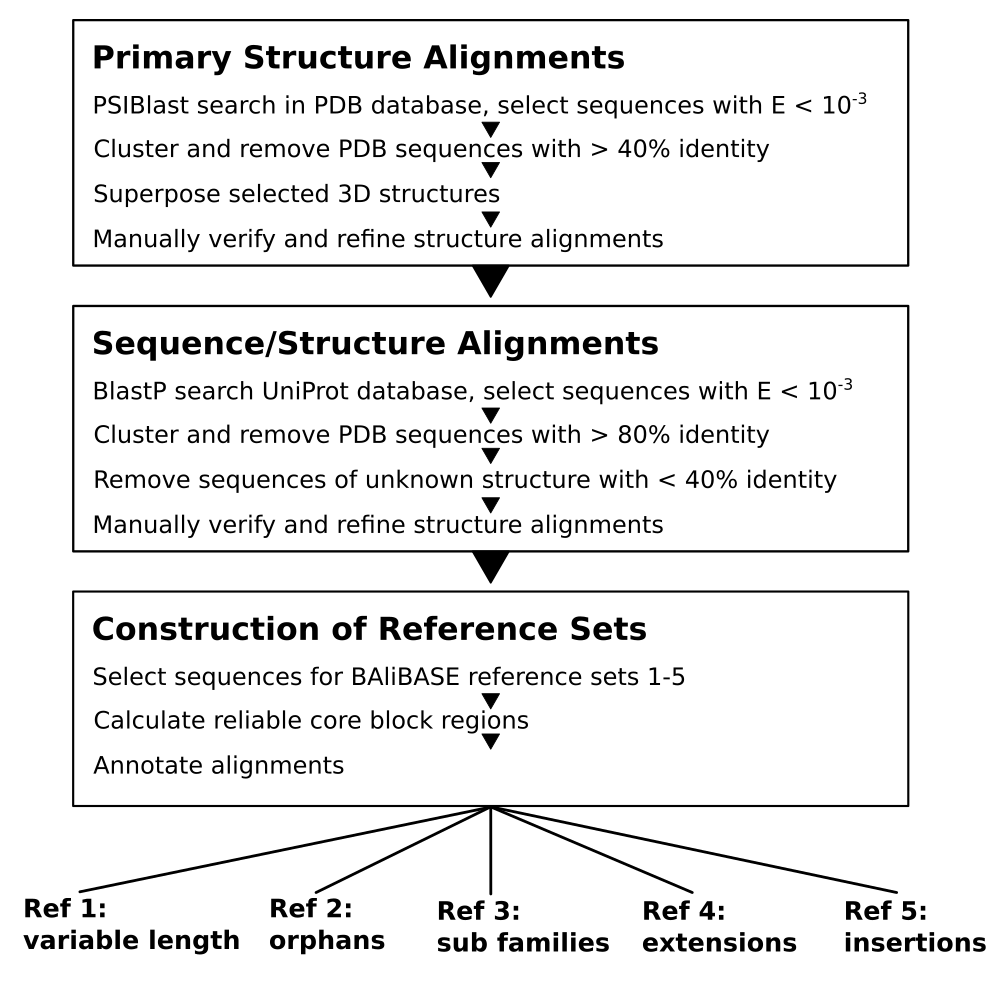
\includegraphics[width=0.5\textwidth]{./images/balibase.png}
	\caption{Flow chart showing the semi automatic process used to establish the reference sets}
	\label{fig:balibase}
\end{wrapfigure}

The third version of the \bb benchmark protein alignment database has been released in 2005 and is widely employed for the comparison of multiple alignment programs \cite{thompson2005balibase, Russell2016}. 



\section{Sum-of-pairs and column score}

\section{MAFFT}

\section{Results}

    \myemptypage


    \chapter{Conclusion}

\section{Further work}

\subsection{Parallelisation Opportunities}

    \myemptypage

    %--- references ---
    \bibliographystyle{IEEEtran}
    \bibliography{content/references}
    \addcontentsline{toc}{chapter}{\bibname}
    \myemptypage

    %--- appendix ---
    \begin{appendix}
        \input{content/appendix_a}
        \myemptypage
    \end{appendix}
    
\end{document}